
\documentclass[a4paper,twoside,openright,12pt,slovene]{book}
\usepackage[pdftex]{UNI-LJ-FE-Diploma} % stil zaključnega dela UL FE
\usepackage[utf8]{inputenc} % predloga uporablja standardno kodiranje Unicode UTF-8, ki podpira šumnike
\usepackage[greek,english,slovene]{babel} % seznam uporabljenih jezikov (zadnji na seznamu je primarni)


\usepackage{filecontents}
\begin{filecontents*}{\jobname.xmpdata}
    \Title{Simulator elektrostatične raztelektritve} % Mora biti enak kot je v prijavi teme!
    \Author{Vid Oblak} % Mora biti enak kot na naslovnici!
\end{filecontents*}
\usepackage[a-1b]{pdfx}
%%%%%%%%%%%%%%%%%%%%%%%%%%%%%%%%%%%%%%%%%%%%%%%%%%%%%%%%%%%%%%%%%%%%%%%%%%%%%%%%%%%%%%%%%%%%%%%%%%%%%%%%%%%%%%%%%%%%%%%%

% LaTeX PAKETI %%%%%%%%%%%%%%%%%%%%%%%%%%%%%%%%%%%%%%%%%%%%%%%%%%%%%%%%%%%%%%%%%%%%%%%%%%%%%%%%%%%%%%%%%%%%%%%%%%%%%%%%%
% Kompakten pregled LaTeX ukazov je dostopen na https://en.wikibooks.org/wiki/Category:Book:LaTeX
% Navodila posameznih uporabljenih paketov so dostopna na https://www.ctan.org

% Dodatni simboli
\usepackage{textcomp}                               % dodatni simboli (kot npr. €)
\usepackage{gensymb}                                % dodatni simboli \de­gree, \cel­sius, \pert­hou­sand, \mi­cro, \ohm
\newcommand{\uppi}{\textrm{\greektext p\latintext}} % velika grška črka P z \uppi, alternativa simbolu \Pi

% Osnovno oblikovanje
\hypersetup{unicode,hidelinks,breaklinks,hyperindex} % dodatne možnosti hiperpovezav
\usepackage[normalem]{ulem}                          % podčrtavanje in prečrtavanje teksta
\usepackage{float}                                   % dodatne možnosti oblikovanja objektov
\usepackage{enumitem}                                % dodatne možnosti oblikovanja seznamov

% Dodatno oblikovanje
%\zamaknirobsodihstrani{0mm} % dodatna prilagoditev levega roba sodih strani za dvostranski tisk
%\usepackage{dcolumn}        % poravnava po decimalnih mestih v tabelah
%\usepackage{longtable}      % večstranske tabele
%\usepackage{caption}        % dodatne možnosti označevanja objektov
%\usepackage{rotating}       % vretenje objektov, strani, ipd.

\usepackage{siunitx} %uporaba SI simbolov

% Matematična orodja
\usepackage{mathtools} % http://mirrors.ctan.org/macros/LaTeX/contrib/mathtools/mathtools.pdf
\usepackage{bm}        % ukaz za odebeljeni tisk \bm v matematičnih okoljih
%\usepackage{cancel}   % ukaz za prečrtavanje \cancel v matematičnih okoljih

% Grafična orodja
\usepackage{graphicx}                 % vključevanje bitnih slik z ukazom \includegraphics
\usepackage{grffile}                  % podpora presledkom pri ukazu \includegraphics
%\usepackage{tikz}                    % paket TikZ za risanje (npr. blokovnih shem, diagramov poteka, itd.)
%\usetikzlibrary{calc,shapes,arrows}  % dodatne možnosti paketa TikZ
%\usepackage{tikzscale}               % skaliranje risb
\usepackage[smartlabels, european, americaninductors]{circuitikz} % risanje shem vezij
%\usepackage{pgfplots}                % paket PGFPlots za risanje grafov, tudi iz CSV in podobnih datotek
%\usepgfplotslibrary{polar,external}  % dodatne možnosti paketa PGFPlots
%\usepackage{tikz-3dplot}             % 3D risanje
% Primeri: http://texample.net , http://pgfplots.net/tikz/examples , http://pgfplots.sourceforge.net/gallery.html

% Vključevanje datotek
\usepackage{pdfpages} % vključevanje PDF datotek z ukazom \includegraphics
\usepackage{epstopdf} % vključevanje EPS datotek z ukazom \includegraphics
\usepackage{listings} % orodja za izpisovanje programske kode
\lstset{              % nastavitve orodja za izpisovanje programske kode
    basicstyle=\ttfamily\footnotesize,
    breaklines=true,
    numbers=left,
    numberstyle=\scriptsize,
    keywordstyle=\color{blue},
    commentstyle=\color{unilj},
    stringstyle=\color{olive},
}
%%%%%%%%%%%%%%%%%%%%%%%%%%%%%%%%%%%%%%%%%%%%%%%%%%%%%%%%%%%%%%%%%%%%%%%%%%%%%%%%%%%%%%%%%%%%%%%%%%%%%%%%%%%%%%%%%%%%%%%%

% DEKLARACIJE %%%%%%%%%%%%%%%%%%%%%%%%%%%%%%%%%%%%%%%%%%%%%%%%%%%%%%%%%%%%%%%%%%%%%%%%%%%%%%%%%%%%%%%%%%%%%%%%%%%%%%%%%%
\naslov{Simulator elektrostatične raztelektritve} % Mora biti enak kot je v prijavi teme!
\avtor{Vid Oblak} % Mora se ujemati s \Title pri metapodatkih PDF/A!
\mentor{Naziv ter ime in priimek mentorja}
%\somentor{Naziv, ime in priimek somentorja}
\date{Ljubljana, \the\year}
\univerza{Univerza v Ljubljani}
\definecolor{unilj}{cmyk}{0.00, 0.94, 0.94, 0.06} % barva Univerze v Ljubljani

\delo{Zaključno poročilo\\~\\Visokošolski strokovni študijski program\\prve stopnje Aplikativna elektrotehnika}
\fakulteta{Fakulteta za elektrotehniko}

% DOKUMENT %%%%%%%%%%%%%%%%%%%%%%%%%%%%%%%%%%%%%%%%%%%%%%%%%%%%%%%%%%%%%%%%%%%%%%%%%%%%%%%%%%%%%%%%%%%%%%%%%%%%%%%%%%%%%
\begin{document}
\frontmatter

\selectlanguage{slovene}

%******************************* NASLOVNICA ************************************
\maketitle

%******************************* ZAHVALA ***************************************
\zahvala
V zahvali se kandidat lahko zahvali mentorju in poimensko tudi vsem sodelavcem in prijateljem, ki so pomagali in prispevali pri delu v laboratoriju, na računalniku, v delavnici, pri tehnični izdelavi dela ali drugje.

%******************************* POVZETEK IN KLJUČNE BESEDE ********************
\povzetek
V tej diplomski nalogi je opisan razvoj simulatorja elektrostatične razelektritve za integrirana vezja. Simulator je sestavljen iz treh glavnih modulov in sicer kontrolne ploščice, nastavljivega visokonapetostnega napajalnika in visokonapetostnega stikala.
Zaradi situacije smo se tekom razvoja projekta odločili da bomo dali povdarek na ugodni ceni. Ta zahteva je pomenila razvoj in izdealvo nastavljivega visokonapetostnega napajalnika in visokonapetostnega stikala, namesto nakupa le teh. 
Vsi moduli projekta so bili načrtovani z modularnostjo v mislih, da v primeru kasnejše nadgradnje ali zamenjave ta poteka čim bolj ne moteno. 

\kljucnebesede
ESD, Elektrostatika, Simulator elektrostatične razelektritve

\selectlanguage{english}

%******************************* ABSTRACT AND KEYWORDS *************************

\abstract
The thesis addresses...

\keywords
ESD, Electrostatic, ESD Simulator

\selectlanguage{slovene}

%******************************* KAZALO ****************************************
\tableofcontents

%******************************* SEZNAM SLIK, SEZNAM TABEL *********************
\seznamslik
\seznamtabel

%******************************* SEZNAM SIMBOLOV *******************************
\seznamsimbolov
V pričujočem zaključnem delu so uporabljene naslednje veličine in simboli:

\begin{center}
    \begin{tabular}{*{4}{l}} \hline
        \multicolumn{2}{c}{\bf{Veličina / oznaka}}           & \multicolumn{2}{c}{\bf{Enota}} \\ \hline
        Ime                & Simbol                          & Ime      & Simbol              \\ \hline
        čas                & $t$                             & sekunda  & s                   \\
        frekvenca          & $f$                             & Hertz    & Hz                  \\
        tlak               & $p$                             & Pascal   & Pa                  \\
        sila vzgona        & $\textbf{\textit{F}}_\text{vz}$ & Newton   & N                   \\
        gostota            & $\rho$                          & -        & kg/m$^3$            \\
        masa               & $m$                             & kilogram & kg                  \\
        vhodna napestost   & $U_\text{vh}$                   & volt     & V                   \\
        Jacobijeva matrika & $\mathbf{J}$                    & -        & -                   \\ \hline
    \end{tabular}
\end{center}

Pri čimer so vektorji in matrike zapisani s poudarjeno pisavo. Natančnejši pomen simbolov ter njihovih indeksov je razviden iz ustreznih slik ali pa je pojasnjen v spremljajočem besedilu, kjer je simbol uporabljen.

\mainmatter

%******************************* UVOD ******************************************
\chapter{Uvod} \label{uvod}

Praktično uposabljanje sem opravljal v podjetju Renishaw d.o.o., podjetje se ukvarja z integriranimi vezji za speficično uporabo (ASIC). Podjetje je bilo ustanovljeno leta kot hčerinsko podjetje Britanskega podjetja Renisahw p.l.c. Zaposleni so razdeljeni na tri skupine:
\begin{itemize}
	\item načrtovalci: načrtujejo posamezne sklope inegriranega vezja in karakterizirajo vezje s pomočjo simulacij.
	\item postavljalci: postavijo posamezne komponente na površino inegriranega vezja (podobno kot risanje tiskanih vezij).
	\item testni inžinerji: karakterizirajo narejena integrirana vezja, načrtujejo testna vezja in skrbijo za testiranje vezij za proizvodnjo.
\end{itemize}
Jaz sem izvajal praktično usposabljanje v skupini testnih inžinerjev. Zadana mi je bila naloga izdelave simulatorja elektrostatične razelektritve, kateri se uporablja pri vertifikaciji integriranih vezij. Zahteve so bile po maksimalni napetosti vsaj \SI{15}{\kilo\volt}, nastavljivost izhodne napetosti med \SI{250}{\volt} in \SI{15}{\kilo\volt}, natančnost izhodne napetosti vsaj 3\% ter ustrezanje CE zakonodaji. 


Za potrebe testiranja integriranih vezij smo v podjetju potrebovali simulator elektrostatične razelektritve. Na začetku snovanja so bile zastavljene specifikacije maximalne napetosti 15kV in uporaba že narejenih modulov za nastavljivi visokonapetostni napajalnik ter visokonapetostno stikalo. Tekom projekta se je to spremenilo in prišlo do odločitve o lastnem načrtovanju nastavljivega visokonapetostnega napajalnika. Pri tem modulu smo imeli kar nekaj tehničnih ovir za prebrosti. Največji sta bili ustrezanje regulacijam CE ter zagotavljanje 15kV izolacije med primarno in sekundarno stranjo.
Prvotni načrti so bili lastno navijanje primernega "step-up" transformatorja. Po kar nekaj mertivah in izračunih se je to pokazalo za neprimerno, saj nismo uspeli zagotoviti željene napetosti in izolacije. Rezervni načrt je bil razdredi televizor s katodno cevjo in iz tam vzeti ven transformator. Tega smo se želeli kar se da izogniti saj se že trenutno težko najde televizorje s katodno cevjo, čez leta se bo pa še težje. Motilo me je pa tudi razlikovanje transformatorjev tako v podnožju kot v karakterisitkah in vgrajene diode v sekundarnem navitju zagotovo ne pomagajo pri karakterizaciji transformatorja. 
Regulacija napetosti nam je povzročala probleme zaradi zagotavljanja željene izolacije. S pomočjo simulacij smo preizkusili kateri tipi krmilnikov bi nam ustrezali. Izločili smo vse neizolirane krmilnike, krmilnik s povratno vezavo preko optičnega spojnika, zaradi nelinearnosti le tega ni bil zmožen pokrivati celotne izhodne napetosti od \SI{250}{\volt} do \SI{15}{\kilo\volt}, krmilnik s povratno vezavo preko pomožnega navitja je v simulacijah izgledal obetavno vendar se je na koncu izkazal za neprimernega. Kot primeren se je izkazal samo regulator ima povratno vezavo preko primarnega navitja in sicer z merjenjem zrcaljene napetosti z sekundarnega navtija na primarno.
%TODO naprej o napajalnikih
Po standardih MIL-STD-883K in JS-001-2007 mora biti visokonapetostno stikalo, katero prazni kondenzator skozi napravo pod testom t.i. "bounce-less" sepravi ko sklene kontakt ga mora zadržati namesto, da ga na krato razklene. Standarda pa tudi predpisujeta obliko signala toka skozi napravo pod testom zato "snubber" vezje čez kontakte stikala ne bi ustrezalo. Za nižje napetosti obstajajo releji kateri vsebujejo živo srebro, katerega naloga je zadržati kontakt, ko se kontakta odbijeta. Vendar takšnega releja za \SI{15}{\kilo\volt} je okoli \texteuro2000.
Kompromis je bil izdelava svojega stikala, katero bo ustrezalo zahtevam.
%jada jada jada o relejih

Princip delovanja simulatorja elektrostatične razelektritve je dokaj enostaven. Nastavljivi visokonapetostni vir polni kondenzator, katerega se nato preko upora prazni skozi napravo pod testom.
\begin{figure}[h]
    \begin{circuitikz}
        \draw (0,0)
       to[V, v=$V$] (0,3)
       to[R=1M] (2,3)
       to[short] (2.685,3)
       to[short] (2.685,2.5);
       
       \draw (3,2)
       node[spdt, rotate=90] {};
       
       \draw (0,0)
       to[short] (3,0)
       to[C=100pF] (3,1.5);
       
       \draw (3,0)
       to[short] (5,0)
       to[short, -d] (5,0.5);
       
       \draw (3.315,2.5)
       to[short] (3.315,3)
       to[R=1500Ohm] (5,3)
       to[short, -d] (5,2.5);
    \end{circuitikz}
          \caption{\label{ESDTesterShemaOsnovna} Osnovna shema ESD simulatorja.}
    \end{figure}

%******************************* POGLAVJA **************************************
\chapter{Simulator elektrostatične razelektritve} \label{ESDSIM}

	\section{Praktično uposabljanje}
	Načrtovalski del projekta, sem delal na svojem računalniškem delovnem mestu, kjer sem uporabljal:
	\begin{itemize}
		\item Altium Designer: risanje električnih shem in načrtovanje tiskanih vezij
		\item Visio: risanje blok diagramov in konceptnih shem
		\item LTSpice: simulacija analognih vezij
		\item STM32Cube: programiranje mikrokrmilnikov ARM STM32
		\item Python: komunikacija med mikrokrmilnikom in računalnikom
	\end{itemize}
	Na mizi sem imel antistatično podlogo, vendar to delovno mesto ni bilo namenjeno meritvam, kvečjem hitrim meritvam, s katerimi sem potrdil koncept.
	Za obsežnejše meritve sem imel na voljo merilno mesto, kjer je bilo tudi na voljo več merilnih inštrumentov. Pri svojem delu sem največ uporabljal:
	\begin{itemize}
		\item Rigol DS1054Z: digitalni osciloskop
		\item neki neki : visokonapetostna diferencialna sonda
		\item Rigol DP832: 3 kanalni laboratorijski napajalnik
		\item PeackTech 3450: multimeter z vgrajeno termalno kamero
	\end{itemize}
	Pred delom z visoko napetostjo, sem moral opraviti interni tečaj varstva pri delu. Po posvetu z mentorjem sva sklenila razdeliti nalogo po posameznih modulih. Za vsak modul sem naprej pripravil blokovno shemo, ter opis možnih rešitev, po pregledu le teh je sledilo nadaljno simuliranje v LTSpice in ko smo bili zadovoljni z rezultati še načrtovanje v Altium Designer.
	
	\section{Zasnova simulatorja elektrostatične razelektritve}
	Poleg že omenjenih specifikacij je veljalo tudi, da mora simulator ustrezati standardoma MIL-STD-883K in JS-001-2007. Osnovna shema simulatorja je sledeča:
	\begin{figure}[h]
    \begin{circuitikz}
        \draw (0,0)
       to[V, v=$V$] (0,3)
       to[R=1M] (2,3)
       to[short] (2.685,3)
       to[short] (2.685,2.5);
       
       \draw (3,2)
       node[spdt, rotate=90] {};
       
       \draw (0,0)
       to[short] (3,0)
       to[C=100pF] (3,1.5);
       
       \draw (3,0)
       to[short] (5,0)
       to[short, -d] (5,0.5);
       
       \draw (3.315,2.5)
       to[short] (3.315,3)
       to[R=1500Ohm] (5,3)
       to[short, -d] (5,2.5);
    \end{circuitikz}
          \caption{\label{ESDTesterShemaOsnovna} Osnovna shema ESD simulatorja.}
    \end{figure}
    
	Sestavljajo ga nastavljivi visokonapetostni izvir, polnilni upor, praznilni kondenzator, praznilni upor ter ne-preskakovalno (t.i. bounce-less) stikalo. Preko polnilnega upora se napolni praznilni kondenzator na željeno vrednost, katerega se v željenem trenutku preko praznilnega upora sprazni skozi napravo pod testom. Izhodni tok mora vstrezati limitam katere so podane v standardih: dvižni čas mora biti manjši kot \SI{10}{\nano\second} ter nominalni čas praznenja kondenzatorja skozi kratki stik mora biti \SI{150}{\nano\second} z maksimalno deviacijo \SI{\pm 20}{\nano\second}. Slednja zahteva pomeni, da z stikalom, povezovalnimi žicami in konektorji smemo dodati maksimalno \SI{20}{\pico\farad}, saj drugače bo čas spraznitve skozi kratki stik odstopal zahtevanemu. Pri načrtovanju visokonapetostnega izvira je prav tako potrebno biti previden, saj mora zagotavljati \SI{15}{\kilo\volt} izolacije med primarno in sekundarno stranjo.

	\subsection{Moduli simulatorja}
	Simulator je sestavljen in 4 modulov, od katerih vsak opravlja posebno nalogo.
	\begin{figure}[h]
    \centering
    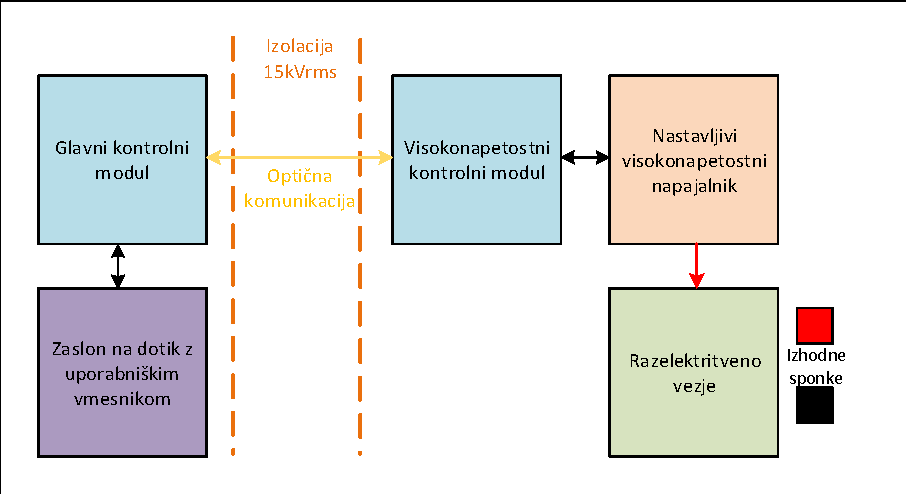
\includegraphics[width=1\columnwidth]{Sheme/Osnovna blok shema poenostavljena.pdf}
    \caption{\label{BlokDiagramShema} Shema blok diagrama.}
	\end{figure}
	
	\begin{itemize}
		\item Glavni kontrolni modul: krmili visokonapetostni modul, prejema uporabnikove ukaze preko zaslona na dotik, pošilja podatke po LAN ali USB
		\item Visokonapetostni kontrolni modul: krmili nastavljivi visokonapetostni napajalnik in razelektritveno vezje po ukazih glavnega kontrolega modula, varnostno odklaplja napajanje nastavljivega napajalnika, ko le ta ni v uporabi
		\item Nastavljivi visokonapetostni napajalnik: po zahtevah regulira napetost od \SI{250}{\volt} do \SI{15}{\kilo\volt}
		\item Razelektritveno vezje: sprazne naboj iz praznilnega kondenzatorja prek naprave pod testom
	\end{itemize}

	\subsection{Nastavljivi visokonapetostni napajalnik}
	Začel sem z nastavljivim visokonapetostnim napajalnikom, saj sem pričakoval, da bo z njim največ dela in na koncu je tudi bilo tako. Z visokimi napetostmi nisem imel nobenih izkušenj, imel sem pa nekaj izkušenj z Cockcroft-Walton-ovim množilnikom napetosti. Hotel sem narediti stikalni napajalnik, kateri bi pretvarjal \SI{24}{\volt} v \SI{250}{\volt} za njim pa 60 stopenj množilnika. Regulaciji napetosti na transformatorju bi sledila tudi izhodna napetost množilnika. Po simulacijah, sem hitro ugotovil, da to ne bo delovalo po pričakovanjih, saj so kapacitivne izgube previsoke. Računi, simulacije koliko dodatnih stopenj blab albllablal. Našel sem pa članek, kjer so se soočali s podobnim problemom ~\cite{Using Parallel High Voltage Multipliers for 100kV Downhole Neutron Generator Power Supplies}, po simulacijah je rešitev izgledala obetavno. Zaradi navdušenja nad rezultati sem se lotil risanja sheme in tiskanega vezja v Altium Designerju. Na srečo smo mojo napako ugotovili, preden smo dali tiskano vezje v izdelavo. Za povratno zanko regulacije sem uporabil analogno-digitalni pretvornik s primerno dimenzinernem preduporom in s tem sem prekinil izolacijo med primarjem in sekundarjem. Sklenili smo, da bo verjetno najboljša možnost za dvigovanje napetosti samo z transformatorjem. Po povpraševanjih pri večjih ponudnikih elektronskih komponent sem prišel do zaključka, da primernega transformatorja ne bo možno kupiti vendar ga bo potrebno narediti. V preteklosti sem že navijal omrežne transformatorje, z načrtovanjem flyback transformatorjev, se pa še nisem srečal. Za začetek sem uporabil jedra RM10 iz materiala N87, katera sem našel v laboratoriju, izračunal sem le koliko obratov rabim na primarni strani, preden preide v nasišenje pri \SI{3}{\ampere}. Navil sem enega z razmerjem 1:10 in enega z 1:20.
%TODO Meritve

Preden sem opravil meritve sem moral narediti še napetostni delilnik za visokonapetostno sondo, saj je le ta narjena samo za \SI{1.8}{\kilo\volt}. Po specifikacijah ima vhodno vpornost \SI{2}{\mega\ohm}, kar pomeni z \SI{18}{\mega\ohm} preduporom, dosežemo razmerje 1:10 in posledično maksimalno napetost \SI{18}{\kilo\volt}. Pri tem je potrebno povdariti, da nisem dodal kapacitivne kompenzacije in sonda je bolj uporabna za indikacijo kot pa meritve. Tuljavo sem krmilnik s pomočjo MOSFETa in namenskega krmilnika UCC27517 proizvajalca Texas Instruments. Zaradi izredno kratkega časa vzpona in padca nam omogoča opravljanje meritve tudi pri višjih frekvencah. Maksimalni izhodni tok \SI{4}{\ampere} nam omogoča hitro odpiranje/zapiranje MOSFETov z višjim \(U_{DS}\). Z signalnim generatorjem sem lahko natančno kontroliral krmilnik. Meritve sem opravljal od \SI{1}{\percent} do \SI{10}{\percent} delovnega cikla, pri napetostih \SI{5}{\volt}, \SI{10}{\volt} in \SI{15}{\volt}. Omejitev toka sem nastavil na \SI{3}{\ampere}, vendar ta ni bila tako pomembna, saj sem imel paralelno iznodnim sponkam vezan še \SI{4700}{\micro\farad} elektrolitski kondenzator. Pri meritvah sem ugotovil, da napetost \(U_pp\) lahko brez problema doseže zahtevanih \SI{15}{\kilo\volt}, vendar se sliši prebijanje napetosti med navitji transformatorja. Odločil sem se narediti meritve še z tremi različnimi jedri. Pri iskanju jedra, sem si pomagal z skripto katero sem napisal v Matlabu, katera mi glede na \(A_L\) in \(l_e\) parametre izračuna potrebno razmerje navojev in maksimalni magnetilni tok. Odločili smo se za nekinekimalitrafo, nekinekiorgormizrežo in nekavelikapizdarija. Večja transformatorja sta izgledala zelo obetavno, saj bi na tuljavniku lažje zagotavljal primerno izolacijo ter visoka \(A_L\) vrednost pomeni manjše število ovojev. Iz radovednosti sem pomeril tudi dva flyback tranformatorja, katera sem naročil kot vzorca od proizvajalca CoilCraft in sicer GA3459 in GA3460, sta pa namenjena za \SI{500}{\volt}. Po mertivah sem prišel do ugotovitev, da transformatorja z velikim jedrom delujeta pod pričakovanji, transformatorja od proizvajalca CoilCraft delujeta izredno dobro in skoraj dosegata željene napetosti najbolje se je izkazal mali transformator z EFD jedrom. 
 
\begin{center}
\begin{tabular}{||c|c|c|c|c|c|c||}
\hline
Ime & \(L_pri\) & \(L_sec\) & Razmerje & \(U_ppMAX\) & Jedro & Reža \\ [0.5ex]
\hline\hline
GA3460 & \SI{2.6}{\micro\henry} & \SI{253}{\micro\henry} & 1:10 & \SI{3.9}{\kilo\volt} & EFD 25/13/9 & \SI{0.5}{\milli\meter} \\
\hline
GA3459 & \SI{5}{\micro\henry} & \SI{505}{\micro\henry} & 1:10 & \SI{13.8}{\kilo\volt} & EFD 25/13/9 & \SI{0.5}{\milli\meter} \\
\hline
Mali z EFD & \SI{76}{\micro\henry} & \SI{13.21}{\milli\henry} & 1:13 & \SI{7.84}{\kilo\volt} & EFD 30/15/9 & \SI{0}{\milli\meter} \\
\hline
\end{tabular}
%\caption{Primerjava podatkov transformatorjev}
\label{table:1}
\end{center}

Z rezultati meritev nisem bil najbolj zadovoljen, vendar sem se odločil najprej ugotoviti način regulacije izhodne napetosti in se kasneje po potrebni prilagoditi parametre transformatorja. 

	\subsection{Regulacija napetosti} \label{RegulacijaNapetosti}
	Prvotno sem si želel skrajšati čas načrtovnja in vzeti že narejeni regulator in po potrebi prilagoditi vezje okoli njega - vezje povratne zanke. Glede na obstoj številnik krmilnikov namenjenih za Flyback topologijo, sem tam začel iskanje primernih, sledeče sem izbral v ožji izbor:
	
\begin{table}[h!]
\centering
\begin{tabular}{||c | c |c||}
\hline
Ime & Proizvajalec & Način povratne zanke \\[0.5ex]
\hline\hline
UCC28740-Q1 & Texas Instruments & Optoizolator \\
LM5155 & Texas Instruments & Optoizolator \\
LT3748 & Linear Technology & Zaznavnje na primarnem navitju \\
LT3757 & Linear Technology & Napetostni delilnik na izhodu \\
LTNEKIBrezFeta & Linear Technology & Zaznavanje na primarnem navitju \\
LTNEKINEKI & Linear Technology & Pomožno navitje \\ [1ex]
\hline
\end{tabular}
\caption{Ožji izbor regulatorjev}
\end{table}

	\subsubsection{UCC28740-Q1} \label{UCC28740-Q1}
Krmilnik ima avtomatsko regulacijo frekvence v obmčju od \SI{170}{\hertz} do \SI{100}{\kilo\hertz}. Povratna vezava je izolirana preko optičnega spojnika, kateri je prožen na izhodni strani preko napetostnega delilnika in Zennerjeve diode. Z spreminjanjem vrednosti upora povratne vezave se spreminja točka, pri kateri se proži optični spojnik. lalalalalaal neki meritve simulacije izračuni kar kol sam da neki je lalalalal

	\subsubsection{LM5155} \label{LM5155}
LM5155 deluje po enakem principu kot že omenjeni UCC28740-Q1.

	\subsubsection{LM3748} \label{LM3748}
Krmilnik je zelo zanimiv, saj ne potrebuje dodatne povratne vezave, informacijo o izhodni napetosti namreč dobi preko zrcaljene napetosti na primarnem navitju. Ko se izključi N Kanalni MOSFET, napetost na ponoru zraste nad vhodno napetost, katera je enaka \(V_{FLBK} = (V_{OUT} + V_F + I_{SEC} * ESR) * N_{PS}) \), ta napetost steče proti masi preko \(R_{FB}\) in interno zaporedno vezanim \(R_{REF}\), točka med uporoma je vezana na ivertirajoči vhod ojačevalnika napake z referenco \SI{1.223}{\volt} \cite{analog:LT3748}. Izhodna napetost je enaka \(V_{OUT} = V_{BG}(R_{FB} / R_{REF})(1 / N_{PS}) - V_F - I_{SEC} (ESR)\), kjer lahko pri naših napetostih zanemarimo \(V_F\) in \(I_SEC (ESR)\), upoštevati pa moramo tudi zahteve za minimalno induktivnost primarnega navitja:
\[L_{PRI} \geq \]

	\subsection{LM3757} \label{LM3757}
Krmilnik LM3757 proizvajalca Linear Technology je krmilnik pri kateremu se nastavlja obratovalno frekvenco z enim uporom v razponu med \SI{100} {\kilo\hertz} in \SI{1} {\mega\hertz}. Napetost se nastavlja z napetostnim delilnikom na sekundarni strani, da pri željeni izhodni napetosti je izhod napetostnega delilnika enak \SI{1.6} {\volt}. Na spletni strani od produkta je bilo možno dobiti vezje regulatorja, katermu sem spremenil vrednosti določenih elementov po mojih potrebah. Po nekaj simulacijah je hitro postalo jasno, da je omenjeni krmilnik primeren za projekt, saj sem uspel nastavljati izodno napetost med \SI{300}{\volt} in \SI{5}{\kilo\volt}. 

    \begin{figure}[H]
        \centering
        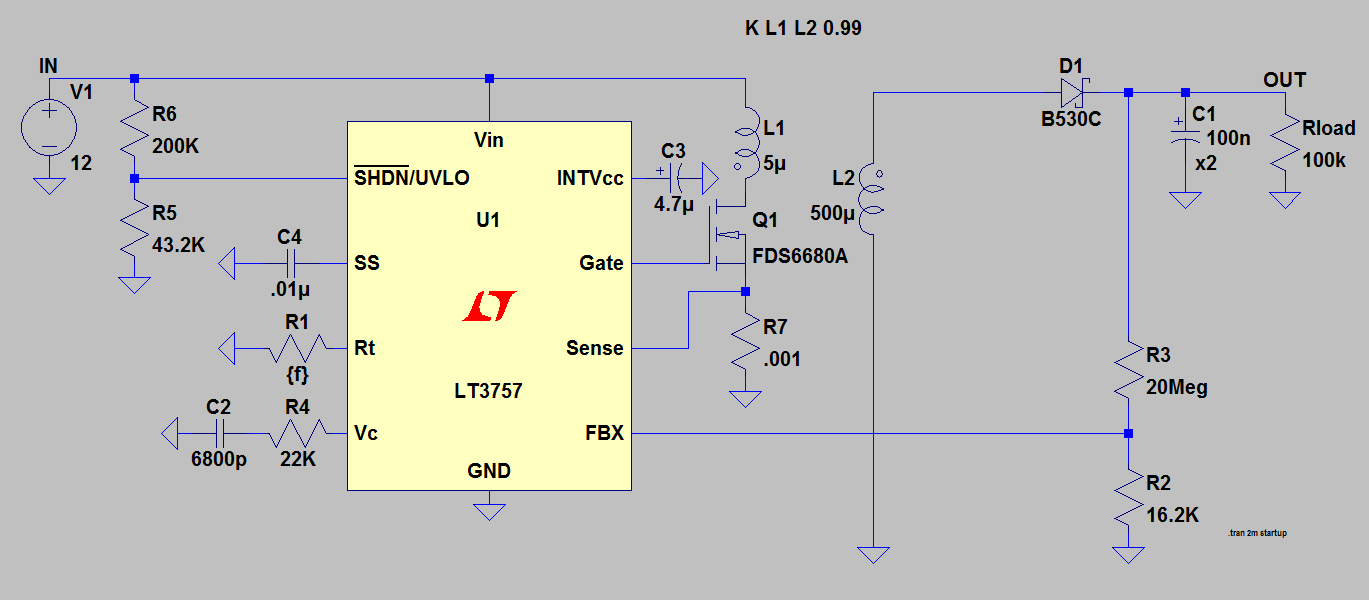
\includegraphics[width=1\columnwidth]{Slike/Simulacije/LM3757spice.png}
        \caption{\label{LM3757spice} Shema vezja v LTSpice.}
    \end{figure}
    
Vendar je problem iz vidika varnosti, sekundarno navitje visokonapetostnega transformatorja je električno povezan z nizkonapetostno stranjo. Za zagotavljanje primerne izolacije bi moral napajalnik modula zdržati \SI{15}{\kilo\volt}, kar zopet pomeni načrtovanje takega napajalnika saj napajalniki z najvišjo prebojno trdnostjo so takšni pod certifikatom IEC 60601-1 po katerem je najvišja prebojna trdnost \SI{4000}{\volt}AC.
    
\chapter{Zahteve} \label{Zahteve}

Pred začetnom snovanja simulatorja elektrostatične razelektritve so bila podane sledeče zahteve:
\begin{itemize}
\item Maksimalna napeost vsaj \SI{15}{\kilo\volt}.
\item Nastavljanje napetosti od \SI{250}{\volt} do \SI{15}{\kilo\volt}.
\item Natačnost izhodne napetosti vsaj 3\%.
\item Avtomatsko preklaplanje med pozitivno in negativno izhodno napetostjo.
\item Možnost spremembe modela razelektritve.
\item Modularna zasnova.
\item Možnost nadgradnje na avtomatični tester.
\item Možnost povezave na LAN.
\item Ustrezanje CE zakonodaji.
\item Ustrezanje standardoma MIL-STD-883K in ESDA JS-001-2017.
\end{itemize}

Tekom projekta so se spremenile sledeče zahteve:
\begin{itemize}
\item Maksimalna napetost vsaj \SI{4}{\kilo\volt}.
\end{itemize}
Ter ni več potrebe po avtomatskem preklapljanju polaritete izhodne napetosti.

\chapter{Blok shema projekta} \label{blokshemaprojekta}

Glavni bloki, kateri sestavljajo simulator elektrostatične razelektritve so:
\begin{itemize}
\item Glavni kontrolni blok,
\item Visokonapetostni kontrolni blok,
\item Nastavljivi visokonapetostni napajalnik ter
\item Visokonapetostno stikalo.
\end{itemize}

\begin{figure}[h]
    \centering
    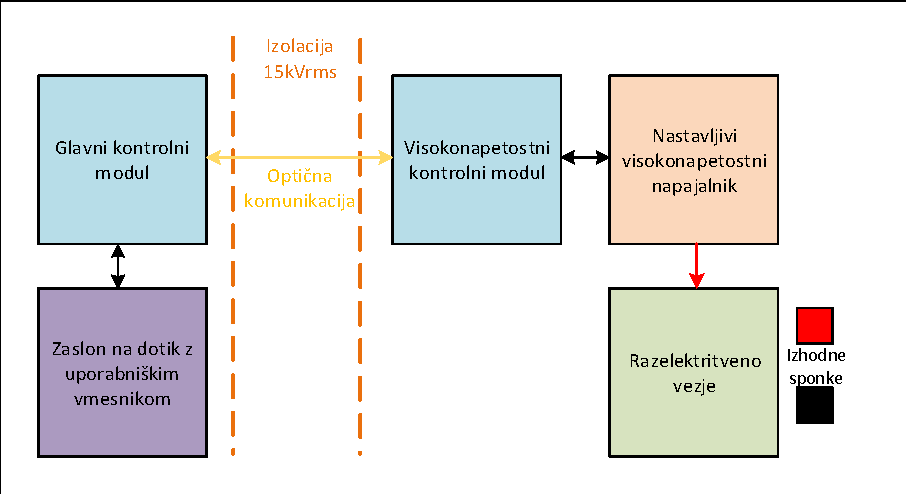
\includegraphics[width=1\columnwidth]{Sheme/Osnovna blok shema poenostavljena.pdf}
    \caption{\label{BlokDiagramShema} Shema blok diagrama.}
\end{figure}



\section{Nastavljivi visokonapetostni napajalnik}

 Nastavljivi visokonapetostni napajalnik, je modul, kateri je verjetno povrožal največ komplikacij. Prvotno je bil plan uporabiti že narjeni modul HP015Z proizvajalca Applied Kilovolts. Omenjeni modul ima maksimalno izhodno napetost \SI{15}{\kilo\volt} in maksimalni tok \SI{400}{\micro\ampere}. Ima možnost nastavitve napetosti glede na napetost na kontrolnem vhodu in možnost izbire pozitivne ali negativne izhodne napetosti. Z uporabo 10 bitnega digitalno-analognega pretvornika (ADC) bi lahko dosegli napetostno resolucijo približno \SI{14,65}{\volt}.
Vendar zaradi takratne situacije je bil zmanjšan proračun za projekt, posledično smo se odločili sami izdelati modul. Specifikacije so ostale enake pri načrtovanju smo se poskušali držati načela, da uporabljamo komponente katere se dobijo pri več različnih virih. Najpomembnejša komponenta je bila transformator. Glede na specfikacij napajalnika je bil najbolj primeren t.i. "flyback" transformator. Želeli smo uporabiti že naviti transformator vendar se je to izkazalo kot nemogoče, saj praktično ne obstajajo takšni, ki imajo nazivno izolacijsko trdnost večjo kot pa \SI{4}{\kilo\volt}. 
Edina možnost katera nam je še ostala je bila lastno navijanje transformatorja. Za prve poizkuse sem uporabil RM10 jedro iz materiala N87, pri prvem primeru sem na primar navil 2 ovoja in na sekundar 20, pri drugem pa na sekundar ovil 40 ovojev. %meritve za narediti bla bla bla
%neki neki neki trafoti
Za krmiljenje MOSFETa sem prvotno uporabljal vezje sestavljeno iz menjalnika nivoja ter "push-pull" komplementarnega para tranzistorjev, katera sta krmilila vrata MOSFETa.

\begin{figure}[h]
    \begin{circuitikz}
        \draw (2,0)
        to[V, v=$Sig$] (2,2)
        to[R=$R_1$] (4,2)
        to[short] (4.5,2);
     
        \draw (5,2) node[npn](npn1){}
        (npn1.base) node[anchor=east, yshift=0.25cm, xshift=0.25cm] {}
        (npn1.collector) node[anchor=south, xshift=0.5cm, yshift=-0.35cm] {}
        (npn1.emitter) node[anchor=north, xshift=0.5cm] {};
     
        \draw (npn1.collector) 
        to[R=$R_2$] (5,5);
        
        \draw (2,0)
        to[short] (5,0)
        to[short] (5,1.5);
     
        \draw (0,0)
        to[V, v=$Vcc$] (0,2)
        to[short] (0,5)
        to[short] (12,5);
     
        \draw (0,0)
        to[short] (12,0)
        to[short] (12,2);
     
        \draw (8,1.5) node[pnp](pnp1){}
        (pnp1.base) node[anchor=east] {}
        (pnp1.collector) node[anchor=north] {}
        (pnp1.emitter) node[anchor=south] {};
     
        \draw (8,3.5) node[npn](npn2){}
        (npn2.base) node[anchor=east] {}
        (npn2.collector) node[anchor=south] {}
        (npn2.emitter) node[anchor=north] {};
     
        \draw (npn2.base)  ++(0,-0.5) node[circ]{};
        
        \draw (pnp1.emitter)   ++(0,-0.275) node[circ]{};
        \draw (pnp1.emitter)   ++(2,-0.275) node[circ]{};

        \draw (5,3) node[circ]{};
        
        \draw (5,5) node[circ]{}; %pike na vcc
        \draw (8,5) node[circ]{};
        
        \draw (5,0) node[circ]{}; %pike na gnd
        \draw (8,0) node[circ]{};
        \draw (10,0) node[circ]{};
     
        \draw (npn2.collector)
        to[short] (8,5);
     
        \draw (pnp1.collector)
        to[short] (8,0);
     
        \draw (5,3)
        to[short] (7.15,3)
        to[short] (7.15,3.5)
        to[short] (7.15,1.5);
     
        \draw (8,3)
        to[short] (8,2)
        to[short] (8,2)
        to[R=$R_3$] (10,2)
        to[R=$R_4$] (10,0);
     
        \draw (12,2.259) node[nigfete](NFET1){};
      
        \draw (10,2)
        to[short] (11.25,2);
     
        \draw (12,3)
        to[L=$L1$] (12,5);  
    \end{circuitikz}
                \caption{\label{BJTFETDriver} Shema MOSFET krmilnika narejena z bipolarnimi tranzistorji.}
    \end{figure}


    Pri meritvah se je pokazalo, da vezje prepočasi odpira MOSFET. Rešitev je bila krmilnik vrat z namenskim čipom UCC27517 proizvajalca Texas Instruments. Zaradi izredno majhnega časa vzpona in padca nam omogoča opravljanje meritev tudi pri višjih frekvencah. Maksimalni izhodni tok \SI{4}{\ampere} nam omgoča hitro odpiranje/zapiranje MOSFETov, kateri so namenjeni za višje moči in napetosti.
 \begin{figure}[h]
        \begin{circuitikz}
            \draw (0,0)
		to[V=Vcc] (0,5.05);
		
		\draw (4,2)
		node[twoportshape] (Q) {}
		(Q.w) node[left] {}
		(Q.e) node[right] {}
		(Q.n) node [above] {UCC37517};
		
		\draw (2,0)
		to[V=Sig] (2,2)
		to[short] (Q.w);
		
		\draw (6,2.28)
		node[nigfete] (fet) {}
		(fet.G) node[anchor=east] {}
		(fet.D) node[anchor=north] {}
		(fet.S) node[anchor=south] {};
		
		\draw (Q.e)
		to[short] (fet.G);
		
		\draw (fet.S)
		to[short] (6,0)
		to[short] (0,0);
		
		\draw (fet.D)
		to[L] ++(0,2)
		to[short] ++(-6,0);
		
		\draw (2,0) node[circ] {};
        \end{circuitikz}
                \caption{\label{KrmilnikUCC27517} Shema krmilnika z UCC27517.}
    \end{figure}
    
~\\Testi so bili narejeni na sledečih transformatorjih:
    \begin{itemize}
    	\item GA3459 proizvajalca CoilCraft
    	
    	\item GA3460 proizvajalca CoilCraft
    	
    	\item Z jedrom RM10 in prestavnim razmerjem 1:10
    	
    	\item Z jedrom RM10 in prestavnim razmerjem 1:20
    	
    	\item Z jedrom EFD 30/15/9 in prestavnim razmerjem 1:13
    	
    	\item in še kr neki drugih trafotov bla bla bla bla
    
    \end{itemize}

GA3459 in GA3460
Transformatorja sta namenjena za uporabo z krmilnikom za polnenje kondenzatorjev LT3751 proizvajalca Linear Technology. Nazivno napetostno območje je \SI{5}{\volt} - \SI{24}{\volt} in nazivna izhodna napetost je \SI{500}{\volt}. Prvotni načrt je bil regulacija izhodne napetosti v območju od \SI{10}{\volt} do \SI{500}{\volt} ter 30 stopenjski paralelni množilnik ~\cite{Using Parallel High Voltage Multipliers for 100kV Downhole Neutron Generator Power Supplies}. Kasneje sem spremenil mnenje in se odločil uporabiti samo transformator za doseganje končne izhodne napetosti. Glede na relativno visoko izhodno moč transformatorja sem se odločil opraviti meritve maksimalne izhodne napetosti, čeprav je nazivna izolacija samo eno minuto pri \SI{1500}{\volt_{rms}}. Čeprav so specificirane maksimalne tokovne špice \SI{20}{\ampere}, sem se pri meritvah omejil na \SI{3,2}{\ampere}. Pri vhodni napetosti \SI{10}{\volt} ter duty cycle 6\% sem dosegel \SI{13.8}{\kilo\volt_{max}} in \SI{9920}{\volt_{pp}}. Vendar se je pri tej napetosti že slišalo šumenje in vohalo po ozonu. Z seciranjem enega transformatorja sem prišel do uporabnih podatkov. Po meritvah jedro ustreza EFD 25/13/9 proizvajalca TDK in je iz materiala N87 z 0,55mm zračne reže ali N97 z \SI{0,5}{\milli\meter} zračne reže. V obeh primerih to pomeni vrednost \(A_{L}=\SI{160}{\nano\henry}\).  Z GA3460 pa rezultati niso spodbujojoči, saj ima induktivnost primarnega navitja za pol manjšo in sicer 2,5uH. Zaradi tega tudi magnetilni tok hitreje naraste do omejitve in posledično je bila najvišja izmerjena napetost \SI{4800}{\volt_{max}} in \SI{3120}{\volt_{pp}}.

    
~\\Transoformatorja z jedrom RM10 sta bila načrtovana glede na tok nasičenja na primarju in razmerja 1:10 ter 1:20 izbrana poljubno. Potrebno je povdariti, da sta bila načrtovana kot navadna transformatorja in ne kot flyback......

~
\\Z jedrom EFD 30/15/9 smo opravljali meritve, saj je zelo podoben temu jedru, ki je v transformatorjih od Coilcrafta. Edina razlika je, da je naše jedro brez zračne reže. 


    
    Pomeril sem pa tudi že narejene flyback transformatorje, kateri so mi ostali od nekega drugega projekta. In sicer GA3459 in GA3460 proizvajalca Coilcraft. Z njima sem dosegal napetosti nekinekineki vendar sta imela nazivno izolacijo samo \SI{1500}{\volt_{rms}}, kar je v praksi pomenilo, da ko je transformator dosegel izhodno napetost približno \SI{10}{\kilo\volt} se je začelo slišati kako prihaja do preboja med navitji.
    Izkazalo se je, da bo potrebno prilagoditi prvotne zahteve in sicer potrebno bo uporabiti transformator, katerega se čedalje težje dobi - flyback transformator iz televizorja s katodno cevjo. Za barvne televizorje so običajno \SI{35}{\kilo\volt} in \SI{40}{\watt}, poleg tega imajo tudi vgrajene visokonapetostne diode. Prvi testi so se izkazali za več kot odlični, saj pri napjalni napetosti \SI{12}{\volt} z delovnim ciklom od 0 do 25\% lahko pokrijemo celotno željeno napetostno območje. Poleg tega je pa tudi magnetilni tok na primarnem navitju precej nižji, kot pa pri alternativah. 
    Nam pa seveda ta rešitev prinese druge probleme. Izredno težko bi bilo dobiti nadomestni transformator kateri ima podobne karakteristike ter enako podnožje. Podatkovnega lista se pa tudi ne dobi, v simulacijah bi bilo v veliko pomoč, če bi imel podano induktivnost sekundarnega navitja. Le to je nemogoče pomeriti z navadnim RLC merilnikom, saj imajo takšni transformatorji med zaporedno vezanimi sekundarnimi navitji visokonapeotne diode. Razmerje med številoma ovojev na primarnem navitju in na sekundarnem navitju bi pa prišlo prav pri izračunih za določene napetostne regulatorje.
    Vendar vseeno prednosti odtehtajo te probleme. 
    Regulacija nam je pa tudi povzročila kar nekaj problemov. Že samo območje regulacije od \SI{250}{\volt} do \SI{15}{\kilo\volt} ni tako majhno, zraven je pa bila tudi želja po meritvi izhodne napetosti in shranjevanju vrednosti le te v povzetek tesiranja. Prvotno sem se zatekel proti že namenskim čipom za regulatorje napetosti, saj bi potreboval samo prilagoditi povratno vezavo. Prve simulacije, katere so obrodile sadove so bile s krmilnikom LT3757. S tem krmilnikom je povratna povezava narejena z napetostnim delilnikom, kateri ni izoliran. Potreben bi bil AC-DC napajalnik, kateri ima prebojno trdnost vsaj 15kV ali baterijsko napajanje za čas polenenja praznilnega kondenzatorja.
    Nobena od teh rešitev mi ni najbolj ustrezala, zato sem simuliral še druge flyback nametostne regulatorje, kateri imajo drugačne načine povratne vezave. Povratna vezava z optospojnikom ni primerna, saj je vseeno potrebno spreminjati vrednost napetostnega delilnika na visokonapetostni strani. Regulacija s pomožnim navitjem je po prvotnih simulacijah izgledala obetavno, ko sem pa popravil vrednosti induktivnosti na vrednosti našega transformatorja se je krmilnik nehal odzivati kot je bilo pričakovano. Zadnja rešitev je bila krmilnik, kateri za povratno vezavo meri zrcaljeno napetost iz sekundarnega navitja proti primarnemu. 
    Simulacije so bile izredno obetavne z krmilnikom LT8304, prav tako meritve opravljene na vezju naspajkanem na prototipni ploščici. Žal je po nekaj časa krmilnik nehal delovati. Naredil sem še enega identičnega, kateri je doživel enako usodo. Predvidevam, da je kriv interni MOSFET, kateri nima načrtovane zaščite za tako visoke zrcalne napetosti kot so v mojem primeru. Na srečo ima proizvajalec Linear Technology v svojem programu tudi krmilnik LT3748 kateri ima povratno vezavo po enakem principu, le da tukaj je zunanji MOSFET, katerega lahko izberemo z primerno visoko maksimalno zaporno napetostjo.
    Izkazal se je za najboljšega kandidata po simlacijah, vendar je potrebno povadati da glede na meritve na transformatorju predvidevam, da ima ta v jedru režo, kar pa je dokaj zahtevno za modelirati zato sem delal simulacije z transformatorjem brez reže. Žal se je izkazalo, da z našim transformatorjem regulacije ne deluje pravilno, saj je neodvisno od vrednostni upora v povarni vezavi krmilnik na vrata MOSFETa pošiljal signal širine približno \SI{55}{\micro\second}, kar je po podatkovnem listu maksimalni čas odprtega MOSFETa. Enačba za izhodno napetost je 
    \begin{equation}
       \\ V_{OUT}=V_{BG}*\left(\frac{R_{FB}} {R_{REF}} \right)*\left(\frac{1} {N_{PS}} \right) - V_{F} - I_{SEC}*(ESR) 
    \end{equation}
    \\Pri tem lahko zanemarimo \(V_{F}\) in \(I_{SEC}*(ESR)\) ter iz podatkovnega lista lahko izločimo, da je \(V_{BG}=1V\). In dobimo sledečo enačbo.
    \begin{equation}
       \\ V_{OUT} = \left(\frac{R_{FB}} {R_{REF}} \right)*\left(\frac{1} {N_{PS}} \right)
    \end{equation}
    \\Za minimalno vrednost primarnega navija je pa sledeča enačba.
    \begin{equation}
       \\ L_{PRI(MIN)} = \frac{\left(V_{OUT} + V_{F(DIODE)}\right) * R_{SENSE} * t_{SETTLE(MIN)} * N_{PS}} {V_{SENSE(NIN)}}
    \end{equation}
    ~\\Pri kateri so podani podatki \(V_{SENSE(MIN)}=\SI{15}{\milli\volt}\) ter \(t_{SETTLE(MIN)}=\SI{400}{\nano\second}\), \(V_{F(DIODE)}\) pa lahko zanemarimo). Za \(R_{SENSE}\) bomo pa uporabili \SI{10}{\milli\ohm}. Druga enačba za minimalno induktivnost primarnega navitja je pa.
    \begin{equation}
        \\ L_{PRI(MIN)} = \frac{(V_{IN(MAX)} * R_{SENSE} * t_{ON(MIN)} * N_{PS}} {V_{SENSE(NIN)}}
    \end{equation}
    \\Pri kateri je podan \(t_{ON(MIN)}=\SI{250}{\nano\second}\). 
    ~\\Razmerja ovojev primarnega in sekundarnega navitja nimamo podanega in zaradi diod v sekundarnem navitju ni ravno enostavno izmeriti sem to vrednost predpostavil. Podatki so \(R_{REF}=\SI{6.04}{\kilo\ohm}\), \(V_{OUT(MAX)}=\SI{15}{\kilo\volt}\), \(V_{OUT(MIN)}=\SI{250}{\volt}\) in \(N_{PS}=0.1\).
    Ko poračunamo enačbe dobimo sledeče rezultate za razpon upora za povratno vezavo \(R_{FB(MAX)}=\SI{9.04}{\mega\ohm}\), \(R_{FB(MIN)}=\SI{151}{\kilo\ohm}\). Za minimalne induktivnosti primarnega navitja \(L_{PRI(MIN)}=\SI{400}{\micro\henry}\) in \(L_{PRI(MIN)}=\SI{2}{\micro\henry}\), upoštevati moramo višjo vrednost sepravi \(\SI{400}{\micro\henry}\).
    Naša transformatorja imata induktivnosti primarnih navitij \SI{411}{\micro\henry} in \SI{330}{\micro\henry}, kar pomeni, da s tem krmilnikom lahko uporabimo samo večji transformator. 
~\\Vendar po 3 poskusih je vedno krmilnik odpovedal. Po približno minuti delovanja ni več kazal znakov življenja. Glede na izmerjenih \SI{0}{\volt} na nogici številka 5, kjer deluje interni linearni regulator predvidevam, da je ta odpovedal in posledično celotni krmilnik ne deluje več. Edina rešitev, katera nam preostane je izdelava svojega krmilnika z mikrokrmilnikom, izoliranim ADCjem ter PID regulatorjem. V tem času so se spremenile zahteve na maksimalno napetost \SI{4}{\kilo\volt} kar nam olajša izbiro komponent. Za ADC sem prvotno hotel uporabiti takšnega, kateri ima že vgrajeno izolacijo naprimer AD7405 proizvajalca Analog Devices. Vendar se nam tu pojavi problem izoliranega napajanja, saj je vseeno potrebno načrtovati napajalnik z transformatorjem, kateri ima vsaj \SI{4}{\kilo\volt} prebojne trdnosti. Rešitev so digitalni izolatorji serije ISOW proizvajalca Texas Instruments. Slednji imajo 4 ali 6 izoliranih digitalnih kanalov ter izolator napetosti. Tako lahko uporabimo normalni ADC, kateri ustreza našim zahtevam in še vedno ustrezamo varnostnim zahtevam glede izolacije.
    
    \chapter{Visokonapetostno stikalo} \label{Visokonapetostno_stikalo}

    Standard zahteva "Bounce-less" stikalo sepravi stikalo, katero ko sklene kontakt ga ne razklene več. Prvotna izbira je bil model G61A proizvajalca Gigavac, kateri se tudi nahaja v simulatorjih elektrostatične razelektritve, saj je v specifikacijah povdarjeno: Odličen za praznjenje kondenzatorjev ter efektivno operira brez "bouncinga".
    Vendar se cena takšenga releja giba okoli 2000\euro{}. Zaradi omejenega proračuna ni bilo mogoče odobriti nakup dotičnega releja. Dobra alternativa se je zdel rele serije H proizvajalca Medler electronics (sedaj Standex electronics) kateri ima v specifikacijah navedeno "Zamenjava za mokre releje z živim srebrom". Pri ceni okoli 50\euro{} se je to zdelo predobro, da bi bilo res.
    Testi so pokazali točno to, kar smo pričakovali: skakanje kontaktov.
    
    \begin{figure}[H]
        \begin{circuitikz}
           \draw (2,1)
            to[V, v=$Sig$] (2,3)
            to[short] (4,3)
            to[L] (4,1)
            to[short] (2,1);
        
           \draw (0,0)
            to[short] (0,1)
            to[C=10nH] (0,3)
            to[short] (0,4)
            to[R=10Ohm] (5,4)
            to[normal open switch] (5,0)
            to[short] (0,0);
    
        \draw (2.5,6) node[oscopeshape](osc1){}
        (osc1.left) node[anchor=west] {}
        (osc1.right) node[anchor=east] {};
        
        \draw (osc1.left)
        to[short] (0,6)
        to[short] (0,4);
        
        \draw (osc1.right)
        to[short] (5,6)
        to[short] (5,4);
        
        \draw (0,4) node[circ]{};
        \draw (5,4) node[circ]{};
	\end{circuitikz}
	   \caption{\label{MerilnoVezjeRele} Shema vezja za merjenje relejev.}
    \end{figure}
    
    \begin{figure}[H]
        \centering
        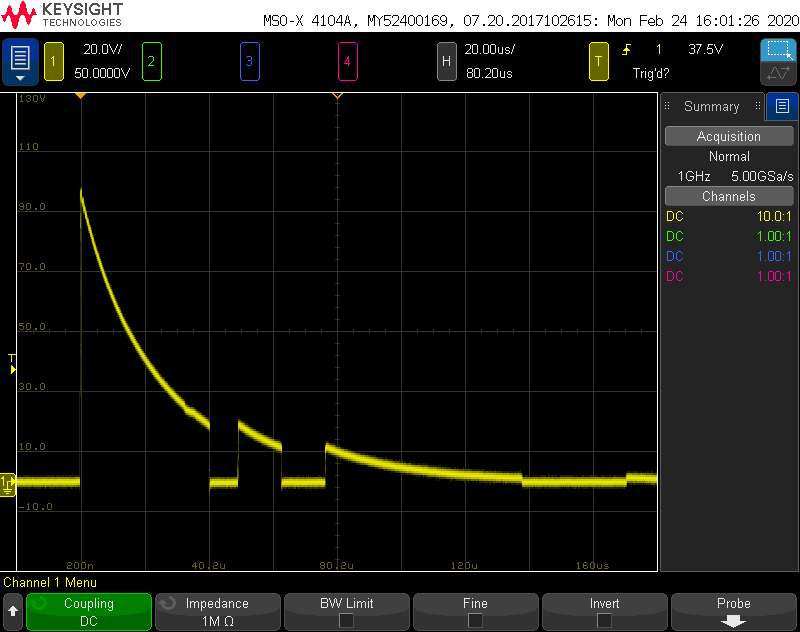
\includegraphics[width=1\columnwidth]{Slike/MedlerElectronicsRele.png}
        \caption{\label{BlokDiagramShema} Skakanje kontaktov pri releju proizvajalca Medler electronics.}
    \end{figure}
    ~\\Po specifikacijah bo največji tok čez rele \SI{10}{\ampere}, saj imamo maksimalno napetost \SI{15}{\kilo\volt} in kondenzator praznimo z \SI{1500}{\ohm} uporom. Zaradi varnosti sem pri merjenju sem spremenil RC konstanto iz \SI{1500}{\ohm} in \SI{100}{\pico\farad} na \SI{10}{\ohm} in \SI{10}{\nano\farad} katero sem napajal iz \SI{100}{\volt}. Na posnetku zaslona iz osciloskopa se lepo vidi razklenitev pri \SI{40}{\micro\second} in \SI{55}{\micro\second}. Po ponovitvah sem ugotovil, da so razklenitve časovno zelo konstantne. Nastala je ideja o vezanju dveh ali več enakih relejev vzporedno in vzbujanje le teh s časovnim zamikom, saj bi tako premostili razklenitev. Vendar bi s tem dodali kapacitivnost v sistem na katero moramo biti zelo pozorni saj standard dovoljuje maksimalno \SI{20}{\nano\second} deviacije časovne konstante kar nanese na \SI{13}{\pico\farad}.
    Iz radovednosti sem naredil meritve še pri višjih napajalnih napetostih vzbujevalne tuljave, kjer sem predpostavljal, da bo magnetno polje dovolj močno, da se kontakt ne bo uspel odbiti. Vendar temu ni bilo tako saj tudi pri trojni napajalni napetosti so se prekitivne še vedno dogajale. 
    
    ~\\Mojo pozornost je pritegnil tudi izdelek podjetja Behlke, katero se ukvarja z visokonapetostno in močnostno elektroniko. Izdelek je bil HTS 181-02-C hitro visokonapetostno tranzistorsko stikalo. Dotični model ima maskimalno napetost \SI{18}{\kilo\volt} ter maksimalno tokovno špico \SI{12}{\ampere}. Malo manj vzpodbudne so številke za čas naraščanja saj v naših primerih bi bile od \SI{12}{\nano\second} do \SI{25}{\nano\second}. Kar je precej več kot \SI{10}{\nano\second} kot jih zahteva standard. Cena takega stikala je okoli 1100\euro , tako da zopet presega naš proračun. Po pregledu fotografij tega stikala in podobnih sem našel sliko, kjer je bil brez pokrova. Najbolj me je zanimal kako je bil izveden visokonapetostni del. Izgleda da uporabljajo več zaporedno vezanih tranzistorjev. Porodila se je ideja o načrtovanju takšnega stikala z komercialno dobavljivimi komponentami.
    Prva ovira je bila izbirane polprevodnikov, kateri so primerni za nalogo. IGBTji IXYL60N450 proizvajalca LittleFuse so se na papirju izkazali za najboljše, saj imajo maksimalno VCES napetost \SI{4.5}{\kilo\volt} vendar imajo tipični odpiralni čas \SI{55}{\nano\second} kar je še vedno 5.5 krat preveč. 
    %preveri spodnjo trditev
    Sem pa našel tranzistorje kateri so bili namenjenei za \SI{10}{\kilo\volt} z risetime okoli \SI{10}{\nano\second}. Tako bi lahko uporabili dva in ju zbondirali na tiskano vezje in s tem zmanjšali parazitne kapacitivnosti in induktivnosti. Vendar zaradi tako hitrega rise timea spadajo te tranzistorji pod Dual use in za nakup le teh potrebno podpisati NDA.
    \\Vendar mi je dalo misliti, če se uporabi najbolj idealne komericalne tranzistorje, jih odstrani iz ohišja, zbondira na tiskano vezje. Kakšne čase bi potem dobili. Preden začnem risati tiskano vezje sem hotel v simulatorju zasnovati še krmilnik. Uporabljeni bi bili IGBTji zato je potrebno krmilno napetost pripeljati med vrata in emitor. V mojem primeru je potencial emitorja navijšega IGBTja proti masi \SI{11.25}{\kilo\volt}. S primernimi visokonapetostnimi stikali bi lahko krmilil na način "Switched Cap".
    %shema swtiched cap
    \begin{figure}[H]
        \begin{circuitikz}
            \draw (0,0)
            to[V, v=$Sig$] (0,3)
            to [short] (1.185,3)
            to[short] (1.185,2.85);
            
            \draw (1.5,2.3)
            node[spdt, rotate=90] (sw1) {}
            (sw1.in) node[left] {};
            
            \draw (1.5,0.7)
            node[spdt, rotate=-90, yscale=-1] (sw2) {}
            (sw2.in) node[left] {};;
             
            \draw (sw1.in)
            to[C] (sw2.in);
           
            \draw  (1.815,0.15)
            to[short] (1.815,0)
            to[short] (4,0)
            to[short] (4,1.5);
            
            \draw (4,2)
		node[nigfetd](Q){}
		(Q.G) node[left] {};
		
		\draw (Q.G) to[short] (3.0145,3)
		to[short] (1.815,3)
		to[short] (1.815, 2.85);
		
		\draw (0,0)
            to[short] (1.185, 0)
            to[short] (1.185, 0.15);    
        \end{circuitikz}
                \caption{\label{SwitchedCapFetDriver} Shema idejne zasnove krmiljenja tranzistorja preko "Switched Cap".}
    \end{figure}
    Naletel sem pa na članek \cite{doi:10.1063/1.1143294} kjer so potrebovali podobno rešitev, ki so jo reševali z transformatorji kateri so imeli 1:1 razmerje in primerno prebojno trdnost. V simulacijah se je rešitev obnesla. V resničnem svetu bi me pa skrbelo, če bi kakšen krmilnik ali tranzistor le malo zakasnil, saj bi takrat prisala celotna napetost na njemu kar bi seveda pomenilo preobremenitev le tega.
    \\V iskanju nadaljnih rešitev to pomeni mehanično rešitev in samo eno stikalo ne zaporene ali vzporedne vezave stikal. Lotili smo se hitrih prototipov štirih stikal:
    \begin{enumerate}
   
        \item  Solenoid, kateri drži razklenjena kontakta, skupaj ju vleče vzmet. Ob prožitvi se obrne polariteta napajanja tuljave solenoida, kateri poleg vzmeti tišči kontakta skupaj.
    \begin{figure}[H]
        \centering
        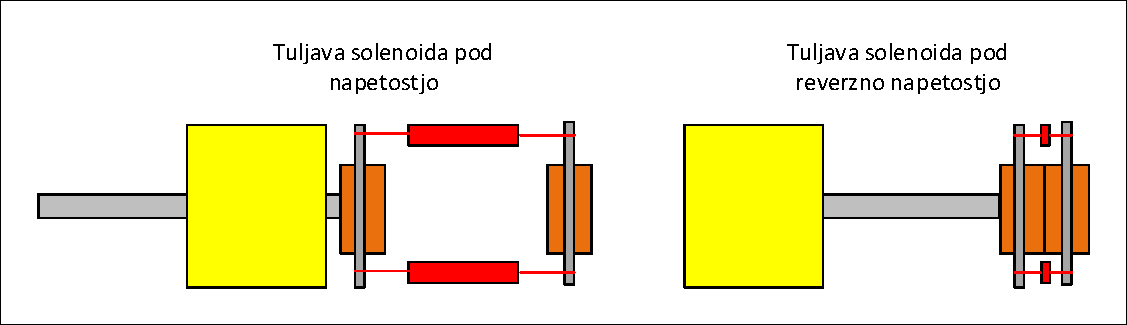
\includegraphics[width=1\columnwidth]{Sheme/StikaloSolenoidVerzija1.pdf}
        \caption{\label{/StikaloSolenoidVerzija1} Shema stikala s solenoidom verzija 1.}
    \end{figure}
    
    \item  Solenoid kateri, porine kontakt in jezička ga ujameta.
    \begin{figure}[H]
        \centering
        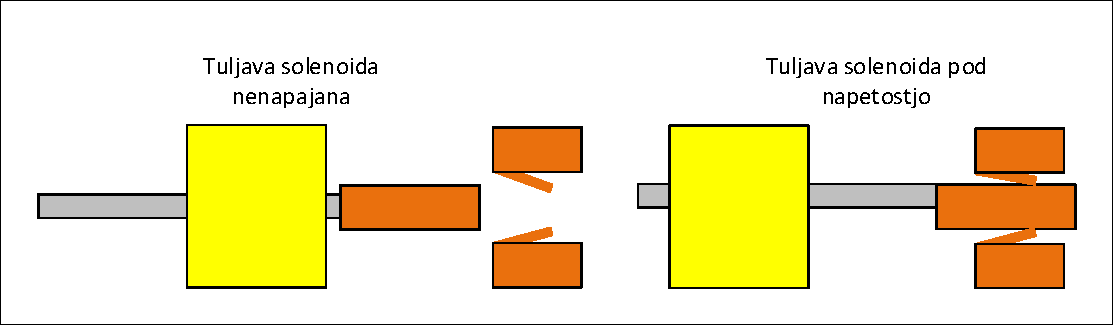
\includegraphics[width=1\columnwidth]{Sheme/StikaloSolenoidVerzija2.pdf}
        \caption{\label{/StikaloSolenoidVerzija2} Shema stikala s solenoidom verzija 2.}
    \end{figure}
    
    \item  Servo motor se zasuče in z drsnim stikalom skelene kontakt.
    \begin{figure}[H]
        \centering
        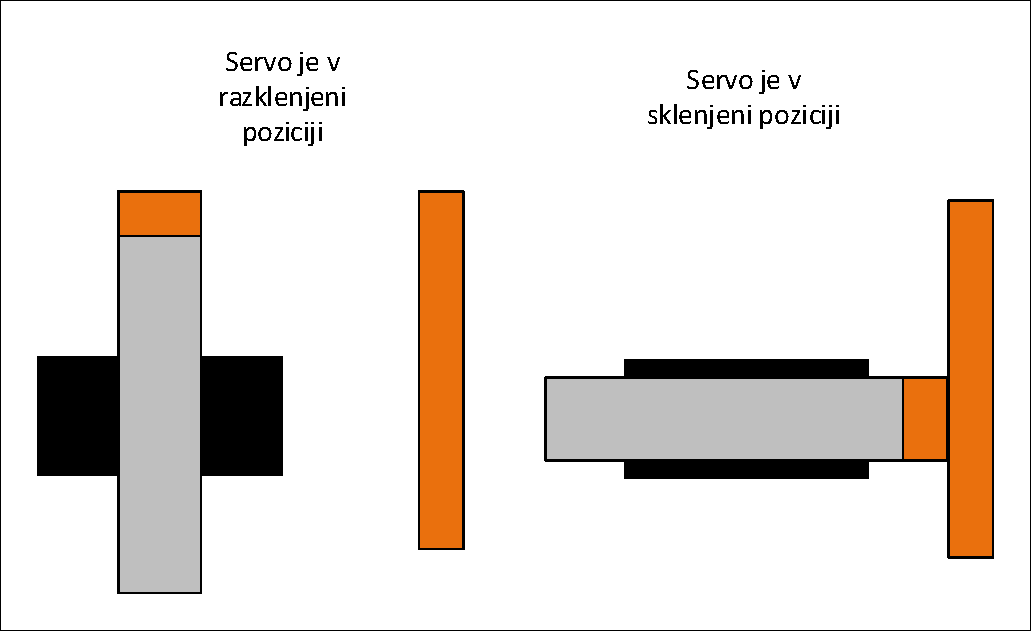
\includegraphics[width=1\columnwidth]{Sheme/StikaloServoVerzija1.pdf}
        \caption{\label{StikaloServoVerzija1} Shema stikala s servo motorjem verzija 1.}
    \end{figure}
    
    \item  Servo motor se zasuče in pritisne na kontakt kateri je na vzmeti.
    \begin{figure}[H]
        \centering
        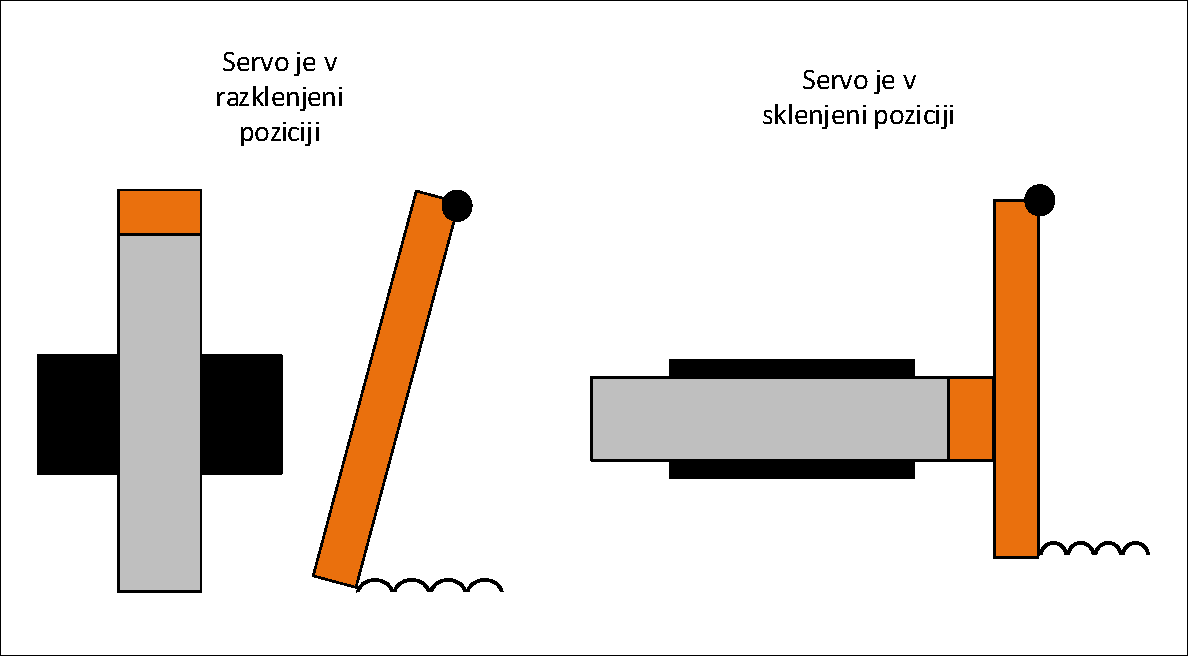
\includegraphics[width=1\columnwidth]{Sheme/StikaloServoVerzija2.pdf}
        \caption{\label{StikaloServoVerzija2} Shema stikala s servo motorjem verzija 2.}
    \end{figure}
\end{enumerate}


    ~\\Za solenoid smo na začetku uporabili manjši model, kateri je bil namenjen konstantnemu delovanju pri \SI{12}{\volt}, za hitrejše delovanje in večjo slilo se ga lahko prenapaja z  \SI{40}{\volt} za čas  \SI{1}{\second} z delovnim ciklom 5\%. Izkazal se je za neuporabnega, saj čim se na njega namesti kontakt nima več zastostne moči za premikanje, posebno če bi se moral še upirati sili vzmeti. Za hitri preiskus mojih tez sem naredil solenoid na tuljanviku od transformatorja.
    %probat še z močnejšim solenoidom
    
    ~\\S stikalo s servo motorjem smo imeli dokaj dobre uspehe vendar smo še vedno bili daleč od končne rešitve. Hitre meritve prototipa stikala z servo motorjem verzija 1 so pokazale rise time  \SI{10}{\nano\second} vendar se vseeno pojavljajo manjše prekinitve po sklenitvi kontaktov. Skrbi me pa tudi obraba in oksidacija kontaktov. Rešitev bi bila zaprtje celotnega stikala v vakumsko komoro ali še bolje $SF_{6}$.
    
    \begin{figure}[H]
        \centering
        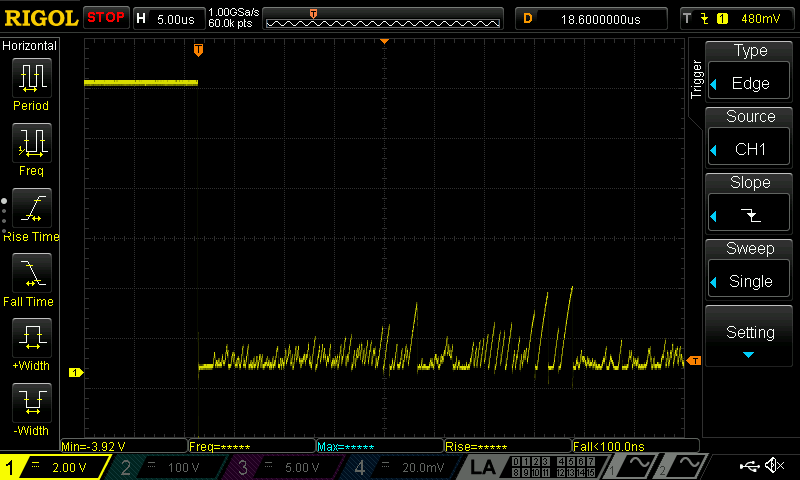
\includegraphics[width=1\columnwidth]{Slike/ServoStikalo1/ServoStikalo1.png}
        \caption{\label{ServoStikalo1} Potek napetosti po sklenitvi kontaktov pri servo stikalu verzija 1.}
    \end{figure}
    
    \begin{figure}[H]
        \centering
        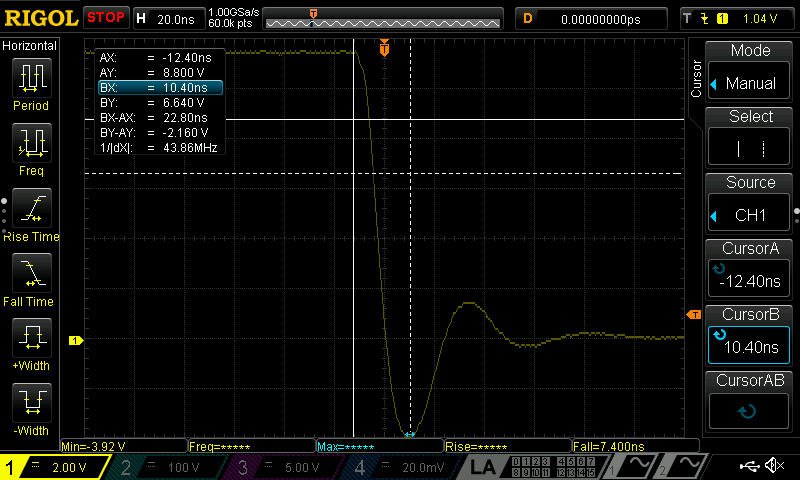
\includegraphics[width=1\columnwidth]{Slike/ServoStikalo1/ServoStikalo1povecano.png}
        \caption{\label{ServoStikalo1povecano} Potek napetosti po sklenitvi kontaktov pri servo stikalu verzija 1 povecano.}
    \end{figure}
    
    ~\\Stikalo s servo motorjem verzija 2 pa je problem počasnega rise tima. Verjetno je kriva vsa parazitna kapacitivnost. Potrebno bi bilo narediti revizijo in skrajšati vse segmente žice in narediti kontakte bolj kompaktne. 
    


\end{document}
%%%%%%%%%%%%%%%%%%%%%%%%%%%%%%%%%%%%%%%%%%%%%%%%%%%%%%%%%%%%%%%%%%%%%%%%%%%%%%%%%%%%%%%%%%%%%%%%%%%%%%%%%%%%%%%%%%%%%%%%
